\subsection{The 3morduc platform}
\label{sec:3morduc}

\begin{figure} [h]
  \begin{center}
    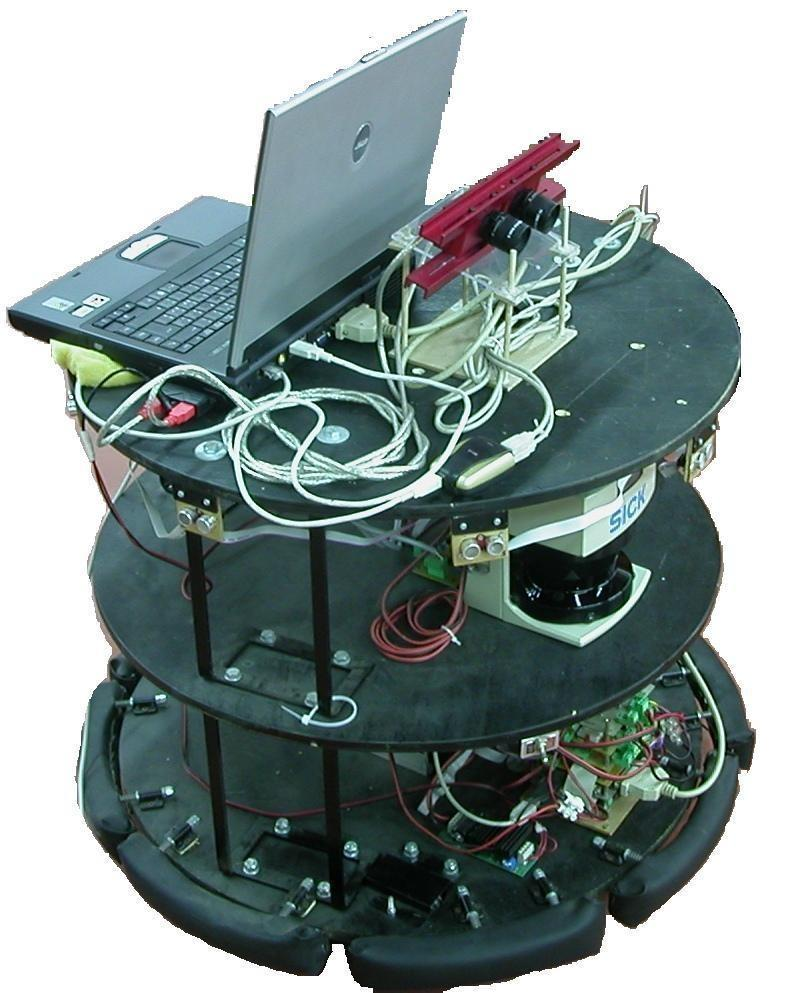
\includegraphics[width=150pt]{img/3morduc.jpg}
    \caption{The 3morduc robotic platform}
    \label{fig:morduc}
  \end{center}
\end{figure}

The telerobot used to develop teleoperation research is
called \textit{3MO.R.D.U.C.}, acronym for `3rd version of
the Mobile Robot DIEES University of Catania'.
3morduc is a mobile-robot, able to move forward, backward
and turn its direction, as directed by the remote operator.
It has been successfully used in several test and experimental
work regarding teleoperation and telepresence.
\\
The robot, actually located at the University of
Catania, is a differential-driven mobile robot, showed
in figure \ref{fig:morduc}.
\\
As every mobile robot, it is equipped with some internal
and external sensors, through which is possible retrieve
information about, respectively, the status of the robot
(e.g. its position) or the data about the environment (e.g.
distance from obstacles).

\subsubsection{Sensors and actuators}
\label{sec:3morduc:sensors_actuators}


The moviment is performed by means of two 40W DC engines, model
\textit{Maxon F2260}, connected with the motor shaft by a gear
box (transmission rate 1/19). On the other side the motor shaft
is linked with two rubber wheels, while a third castor wheel can
freely turn to realize the differential-driven model.
\\
The robot is compound by three shelves, each one connected to
the next. On the lower level two lead batteries are situated,
able to erogate 12 Volts at 18 Amperes. The electrical autonomy is
granted for 30-40 minutes.

\begin{figure}
  \begin{center}
    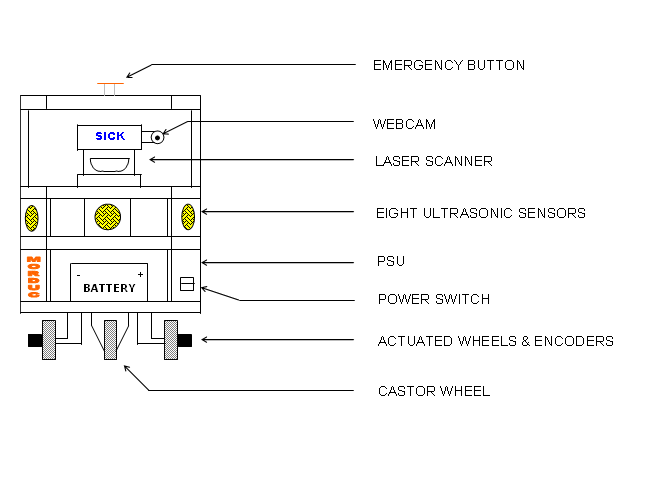
\includegraphics[width=300pt]{img/Morduc_scheme.png}
    \caption{3morduc's schematic figure}
    \label{fig:morduc_scheme}
  \end{center}
\end{figure}

Besides, on the same lower level is located an electronic board
controlling different modules, each one predisposed to manage a
specific task as movements, sensors and communication.
\\
Type and number of sensors avaible on 3morduc are:

\begin{itemize}
\item \texttt{belt of bumpers} \\
  A belt of bumpers (in total 16 switches) is dislocated around
  the entire perimeter on the robot base, just over the wheels level.
  The bumpers are simple switches pushed when there is a collision.
  \\
  These sensors recognize clashes between robot and other objects,
  other then reduce damage in case of a collisions.

\item \texttt{incremental encoders} \\
 The two robot motor axes are equipped with incremental encoders, with
 resolution of 500 pulses per turn. These sensors are useful to calculate
 heading and position of the robot by using the kinematic model.  
 \\
 A rotary encoder is shown in figure \ref{fig:encoder}. For more details
 see \ref{sec:3morduc:encoder}.

\item \texttt{belt of sonars} \\
  On the second level are located eight sonar sensors, which measure the
  distance from an obstacle using the flight time of an ultrasonic signal
  produced by means of a vibrating piezoelectric sensor. 
  For more details about sonar sesors see \ref{sec:3morduc:sonar}.

\item \texttt{scanner laser} \\
  In order to detect obstacles on the workspace, the Laser Measurement
  Sensor (LMS) operates by measuring the flight time of a pulsed laser
  light beam that is reflected by obstacle. An internal rotating mirror
  deflects the transmitted pulsed laser beam so that a scan of the
  surrounding area is made. The returned beams is detected by the laser
  receiver. It is possible to configure different angular resolution
  (0.25, 0.5 or 1 degree pace) with different angular scan (100 or 180
  degrees).
  \\
  The time between transmission and reception of the light pulse is directly
  proportional to the distance between the scanner and the object. 
  Further details about LMS can be found in \ref{sec:3morduc:laser}.

\end{itemize}



\begin{comment}

  una stereocamera STH-MDCS2-VAR-C è posta sul top del robot e connessa al PC mediante
●
  l'interfaccia IEEE 1394. Essa è composta da due camere, ciascuna con risoluzione di 1.3
  Megapixel. Il sensore CCD di queste camere ha una buona immunità al rumore e sensibilità.
  Tuttavia è possibile regolare tutti i parametri dell'immagine (exposure gain, frame rate,
  resolution...). Le due camere sono montate su un supporto rigido che permette di regolarne
  la distanza fra loro in un range di 5-20 cm. Le immagini provenienti dalle due camere sono
  sincronizzate ad una frequenza di 8 Khz [5] [6].

On the robot there are also two high quality stereoscopic cameras; each one has a resolution of 1.3 Megapixel; they are equipped with fixed focus lens of 4.0 mm.
The CCD sensors of these cameras have a good noise immunity and sensibility; moreover, it is possible to adjust all the image parameter, e.g.
exposure gain, frame rate, resolution. The cameras are mounted on a rigid support; it permits to simply adjust the camera distance in a range 5-20 cm.






\end{comment}


More images, video and information about 3morduc can
be found in \cite{morduc:features}.


\subsubsection{Internet communication}
\label{sec:3morduc:communication}
